\subsection{Planeación}\label{subsec:planeacion}
En esta etapa, se estableció el propósito general de la investigación y se definieron las metas, así como las preguntas de investigación, métricas, criterios de clasificación, criterios de inclusión/exclusión y criterios de calidad de los estudios. Ver Figura~\ref{fig:etapa1}.

\begin{figure}[htbp]
    \centering
    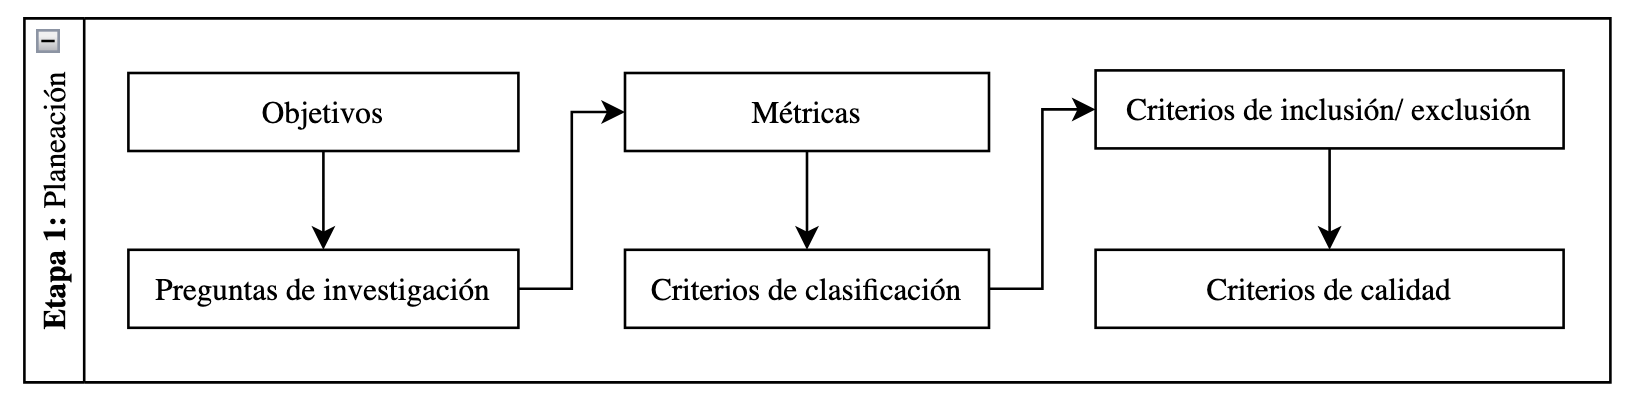
\includegraphics[width=0.5\textwidth]{resources/images/planeacion/etapa1.png}
    \caption{Composición de la etapa de planeación}\label{fig:etapa1}
\end{figure}

\subsubsection{Objetivos}
\mbox{}\\
Teniendo en cuenta los aspectos descritos en la sección de motivación, se definieron 2 metas generales para la revisión sistemática de la literatura que se presentan en el cuadro~\ref{tab:metas}.

\begin{table}[htbp]
    \centering
    \begin{tabular}{>{\centering\arraybackslash}m{1cm} >{\arraybackslash}m{7cm}}
        \hline
        \textbf{Goal} & \textbf{Description} \\
        \hline\\
        M1 & Identificar trabajos relacionados con VBC en proyectos de docencia, investigación y extensión. \\
        \\
        M2 & Clasificar trabajos relacionados con VBC en los dominios de desarrollo de software, pensamiento computacional, computación paralela, análisis de datos, inteligencia artificial, redes computacionales, infraestructura de TI, HPC, entre otros. \\\\
        
        \hline
    \end{tabular}
    \caption{Metas del estudio}\label{tab:metas}
\end{table}

\subsubsection{Pregunta de investigación}
\mbox{}

\begin{table}[tbp]
    \scriptsize % reduce tamaño del texto
    \centering
    \renewcommand{\arraystretch}{1.3}
    \begin{tabularx}{\columnwidth}{>{\centering\arraybackslash}m{0.18\columnwidth} >{\RaggedRight\arraybackslash}X}
        \hline
        \textbf{Aspecto} & \textbf{Descripción} \\
        \hline
        Población & Trabajos relacionados con la VBC aplicadas en diversos dominios de TI con un énfasis en la educación, investigación y extensión. \\
        Intervención & Identificación y clasificación de los trabajos en VBC en los dominios de TI establecidos. \\
        Comparación & 
        1. Se comparan los proyectos que han hecho uso de la VBC para determinar cuáles han tenido mayor tasa de éxito expresado por los autores en cada dominio de TI. \newline
        2. Se analiza el impacto de la VBC en proyectos de docencia, investigación y extensión en comparación con otras soluciones tecnológicas. \\
        Salida & Estructura de clasificación de los trabajos relacionados con las VBC en cada dominio de TI que han impactado en proyectos de docencia, investigación y extensión. \\
        Contexto & Docencia, investigación y extensión con apropiación de los dominios de TI en forma de VBC. \\
        \hline
    \end{tabularx}
    \caption{Aspectos del modelo PICOC}\label{tab:PICOC}
\end{table}

\begin{table*}[!t]
\centering

\renewcommand{\arraystretch}{1.4}
\begin{tabularx}{\textwidth}{>{\centering\arraybackslash}m{0.05\textwidth} >{\centering\arraybackslash}m{0.05\textwidth} >{\RaggedRight\arraybackslash}X >{\RaggedRight\arraybackslash}X}
\toprule
\textbf{Meta} & \textbf{Pregunta} & \textbf{Descripción} & \textbf{Motivación} \\
\midrule
G1 & Q1 & ¿Cuáles son los trabajos relacionados con tecnologías de virtualización basadas en contenedores que podrían impactar positivamente proyectos de docencia, investigación y extensión? & La transversalidad que ofrece la VBC, gracias a su reproducibilidad de entornos, permite estimular diferentes aristas de la sociedad. Su naturaleza facilita el transporte de soluciones de TI entre diferentes entornos, generando que una innovación en cualquier dominio social impacte directamente en otro. \\
\midrule
G2 & Q2 & ¿Cuáles son los principales trabajos relacionados con las tecnologías de virtualización basadas en contenedores que podrían contribuir en los diversos dominios de TI, entre los que pueden ser desarrollo de software, pensamiento computacional, computación paralela, análisis de datos, inteligencia artificial, redes computacionales, infraestructura de TI, HPC, entre otros? & Se busca proporcionar una base sólida para investigadores, docentes y profesionales interesados en comprender el estado del arte actual en relación con las VBC, además del alcance y las aplicaciones de estos trabajos sin necesidad de un análisis profundo. \\
\bottomrule
\end{tabularx}
\caption{Preguntas de investigación y su motivación}\label{tab:preguntas}
\end{table*}
Para la construcción de las preguntas de investigación (RQ, por sus siglas en inglés) se utilizó GQM \textit{(Goal Question Metric)}~\cite{Needleman2002} y el modelo PICOC~\cite{petticrew2008systematic}.
Este modelo permite establecer aspectos como ``Población'', ``Intervención'', ``Comparación'', ``Salida'' y ``Contexto'' que sirven para situar el trabajo a realizar. Ver cuadro~\ref{tab:PICOC}. \\

Teniendo en cuenta la información del modelo PICOC, se definieron 2 RQ. Ver cuadro~\ref{tab:preguntas}.\\
\subsubsection{Métricas}
\mbox{}\\
Se establecieron las métricas del estudio mediante un enfoque cuantitativo, conforme a la estructura de clasificación. Los detalles de dichas métricas se presentan en el cuadro~\ref{tab:metricas}.
Los criterios definidos limitaron la validez de los documentos a un periodo de tres años, con el fin de favorecer la actualidad del estudio.
Asimismo, el tipo de fuente se restringió a estudios primarios, con el propósito de asegurar un mayor rigor en la revisión por pares.

\begin{table}[htbp]
\centering
\renewcommand{\arraystretch}{1.3}
\begin{tabularx}{\columnwidth}{>{\centering\arraybackslash}m{0.15\textwidth} >{\RaggedRight\arraybackslash}X}
\toprule
\textbf{Métrica} & \textbf{Descripción} \\
\midrule
M1 & Cantidad de trabajos identificados en cada dominio de TI. \\
M2 & Cantidad de trabajos que están incluidos en educación. \\
M3 & Cantidad de trabajos que están incluidos en investigación. \\
M4 & Cantidad de trabajos que están incluidos en extensión. \\
\bottomrule
\end{tabularx}
\caption{Métricas definidas para el análisis}\label{tab:metricas}
\end{table}
\subsubsection{Tópicos de investigación}
\mbox{}\\
Las preguntas de investigación y el modelo PICOC sirven como línea base para definir los tópicos considerados relevantes en el estudio. Estos tópicos son: \textit{Container-based virtualization}, \textit{Education}, \textit{Research}, \textit{Industry}. 
La definición de los tópicos de investigación se realizó teniendo en cuenta los dominios de TI que se consideraron relevantes para el estudio.\\

\subsubsection{Criterios de inclusión y exclusión}
\mbox{}\\
\begin{table*}[!t]
\centering
\renewcommand{\arraystretch}{1.4}
\begin{tabularx}{\textwidth}{>{\centering\arraybackslash}m{0.15\textwidth} >{\RaggedRight\arraybackslash}X >{\RaggedRight\arraybackslash}X}
\toprule
\textbf{Categoría} & \textbf{Inclusión} & \textbf{Exclusión} \\
\midrule
Campos & Resumen & --- \\
\midrule
Tipo de publicación & Artículos publicados en revistas científicas o académicas y actas de congresos & Tesis y capítulos de libros \\
\midrule
Área/Disciplina & Gestión de TI, Ciencias de la Computación, Tecnología de la Información y Gestión, Ingeniería & Áreas no relacionadas con virtualización, Ciencias de la Computación, e Tecnología de la Información y Gestión \\
\midrule
Período & Entre 2022 y 2024 & Menos de 2022 \\
\midrule
Idioma & Inglés & --- \\
\bottomrule
\end{tabularx}
\caption{Criterios de inclusión y exclusión}\label{tab:criterios}
\end{table*}
Los criterios de inclusión y exclusión se definieron para propiciar que los estudios seleccionados fueran relevantes para las preguntas de investigación y los objetivos del estudio. Los criterios se presentan en el cuadro~\ref{tab:criterios}.\\
Se estableció un período de 3 años con el propósito de favorecer la actualidad de los estudios. Además, se restringió la selección a artículos de revistas con el fin de promover un mayor rigor en la revisión por pares. Los estudios debían estar escritos en inglés y en las áreas de \textit{Computer Science} y \textit{Management}, \textit{Information Technology and Management}, \textit{Engineering} en aras de mantener la calidad de la muestra. Finalmente, se excluyeron los estudios que no estuvieran relacionados con la VBC, que no hubieran sido revisados por pares o que no estaban disponibles en línea.\\

\subsubsection{Criterios de calidad}
\mbox{}\\
Para finalizar la etapa de planeación, se definieron tres criterios de calidad. \\

El primer criterio de calidad es una adaptación del CVI \textit{(Content Value Index)}~\cite{almanasreh2019evaluation} y~\cite{yaghmaei2003content}.
En este caso, los artículos se evaluaron para determinar si cumplen con los criterios de inclusión y exclusión definidos y si son relevantes para las preguntas de investigación. Se usó una escala cuantitativa de 0 a 5, donde 0 indica una baja relación con las metas del SMS y 5 indica una alta relación.
Ver formula~\ref{eq:cvi}. En esta formula, \textbf{K} es el número impar de evaluadores y \textbf{\textit{f (n)}} es la frecuencia de respuestas para cada valor de la escala.\\

\begin{equation}
\label{eq:cvi}
CVI = \frac{\sum_{n=1}^{k} f(n)}{k}
\end{equation}

El segundo criterio de calidad es el número de citas de cada estudio de acuerdo con la fecha de publicación (\textbf{A}), el cual se denomina SCI \textit{(Scientific Citation Index)}. Ver formula~\ref{eq:sci}. En esta formula, \textbf{C} es el número de citas entre 2022 y 2024 y \textbf{A} es el tiempo de publicación del estudio. Así, un artículo publicado en 2024 con las misma cantidad de citas que un artículo publicado en 2022 tendrá un SCI más alto.\\

\begin{equation}
\label{eq:sci}
SCI = \frac{C}{A}
\end{equation}

El tercer criterio de calidad corresponde a la relación de los estudios con las preguntas de investigación. Este criterio se denomina IRRQ \textit{(Index of Relationship to Research Questions)}. Ver formula~\ref{eq:irrq}.

\begin{equation}
\label{eq:irrq}
IRRQ = \frac{N}{2}
\end{equation}

\textbf{N} corresponde al número de preguntas de investigación que el estudio responde. Este valor se divide en 2 porque es el número de preguntas de investigación definidas en la etapa de planeación.\\